\documentclass{article}
\usepackage[utf8]{inputenc}
\usepackage[english]{babel}
\usepackage{lastpage}
\usepackage{float}
\usepackage{natbib}
\usepackage{graphicx}
\usepackage[margin=1.1in]{geometry}
\usepackage{listings} 
\usepackage{watermark}
\usepackage{blindtext}
\usepackage{amsmath}
\usepackage{amssymb}
\usepackage{footnote}
\usepackage{caption}
\usepackage{textcomp}
\makesavenoteenv{table}
\usepackage[table,xcdraw,svgnames]{xcolor}
\usepackage[bottom]{footmisc}
\usepackage{subcaption}
\usepackage[justification=centering]{caption}
\usepackage{subfiles}
\usepackage{mcode}
\usepackage{enumerate}
\usepackage{wrapfig}
\usepackage{fancyhdr}
\usepackage{hyperref}
\usepackage{bm}
\usepackage{makecell}
\usepackage{changepage}
\renewcommand{\baselinestretch}{1.4}
\newcommand{\ts}{\textsuperscript}
\pagestyle{fancy}

%%% DAVIDs tilføjelser:
\bibliographystyle{ieeetr}
\setlength{\parindent}{0pt}
% Bibliography (references)
\usepackage[backend=biber,
            %backref=true,
            abbreviate=false,
            sortcites=ynt,
            sorting=nyt,
            dateabbrev=false,
            alldates=long]{biblatex}
\addbibresource{references.bib}
%\lhead{Scientific Computing}

\rhead{02686 Scientific Computing for Differential Equations}


\linespread{1.3} % Line spacing

%\setlength\parindent{0pt} % Uncomment to remove all indentation from paragraphs

\graphicspath{{./Fig/}} % Specifies the directory where pictures are stored

\usepackage{geometry}
 \geometry{
 a4paper,
 total={170mm,257mm},
 left=30mm,
 right=30mm,
 top=30mm,
 bottom=20mm
 }
 
\begin{document}

%\renewcommand{\headrulewidth}{0.4pt} %header


\cfoot{\thepage\ of \pageref{LastPage}}
%-------------------------------------------------------------------------------
%	TITLE PAGE
%-------------------------------------------------------------------------------
\begin{titlepage}

\newcommand{\HRule}{\rule{\linewidth}{0.5mm}} % Defines a new command for the horizontal lines, change thickness here

\center % Center everything on the page

\includegraphics[width=0.15\textwidth]{Logo/DTU-logo.pdf}
%\quad \quad \quad \quad \quad
%\includegraphics[width=0.2\textwidth]{KUlogo.png}
\\[1cm]


\textsc{\large 02686 - Scientific Computing for Differential Equations }\\[0.5cm] % Minor heading such as course title

%\textsc{\large \bfseries Tennis Major Tournament Match Statistics}\\[0.5cm]

\HRule \\[0.8cm]
{ \huge \bfseries Comparison of Numerical Solvers
}\\[0.4cm] % Title of your document
\HRule \\[1cm]

\begin{minipage}{0.4\textwidth}
\begin{center} \footnotesize
\emph{Author:}\\
David Ribberholt Ipsen (s164522)\\
\end{center}
\end{minipage}\\[4cm]

{\large 
\today %dato 
}
\\[0.2cm] % Date, change the \today to a set date if you want to be precise
\thiswatermark{\centering \put(-180,-720){\includegraphics[scale=0.55]{Logo/DTU-frise-SH-15.pdf}} }
\end{titlepage}

\newpage
\tableofcontents

\newpage

%-------------------------------------------------------------------------------
%	Problem statement
%-------------------------------------------------------------------------------
\section{Test equation for ODEs}
Considering the test equation

$$
\dot{x}(t)=\lambda x(t), \quad x(0)=x_{0} \label{eq:test}
$$
for $\lambda=-1$ and $x_{0}=1$.

\subsection{Analytical solution}
It is is function that differentiated gives itself times a constant. Therefore try a guess with:
$$
x(t) = \exp(\lambda t)
$$
Then
$$
x'(t) = \lambda \exp(\lambda t) = \lambda x(t)
$$
I.e. the analytical solution is $x(t) = \exp(\lambda t)$.

\subsection{Local and global truncation error}
In order to calculate the local and global truncation error, the analytical, exact solution to the ODE is required to be known. For that reason, the \textit{test equation} is typically used to \textit{test} the performance of numerical methods. The errors are calculated as follows \cite{JrgensenScientificEquations}:
\\

\textbf{Global error}
$$
e_{k}=x_{k}-x\left(t_{k}\right)
$$
where $x_{k}$ is the numerical (descretized) solution and $x\left(t_{k}\right)$ is the exact (continuous) solution. The global error is thus the accumulated error over time. Therefore, it is commonly calculated in the last step.
\\

\textbf{Local error}
$$
l_{k}=x_{k}-x_{k-1}\left(t_{k}\right)
$$
where $x_{k}$ is the numerical solution and $x_{k-1}\left(t_{k}\right)$ is the analytical one-step solution starting from $x\left(t_{k-1}\right)=x_{k-1}$. Therefore, it is commonly calculated in the first step.
\\

Now, it is of interest to calculate the error of the following three methods
\\

\textbf{Explicit Euler \cite{JrgensenScientificEquationsb}}
\begin{equation}
    x_{k+1}=x_{k}+\Delta t f\left(t_{k}, x_{k}\right)
\end{equation}

Which intuitively takes a step forward with the current $\dot{x}(t_k)$.
\\
\textbf{Implicit Euler \cite{JrgensenScientificEquationsb}}
\begin{equation}
    x_{k+1}=x_{k}+\Delta t f\left(t_{k+1}, x_{k+1}\right)
\end{equation}

Which intuitively takes a step backward with the following $\dot{x}(t_{k+1})$ as estimated by Newton's Method [ibid.].
\\
\textbf{Classical Runge-Kutta \cite{JrgensenRunge-KuttaEquations}}
$$
\begin{aligned}
T_{1} &=t_{n} & X_{1} &=x_{n} \\
T_{2} &=t_{n}+\frac{1}{2} h & X_{2} &=x_{n}+h \frac{1}{2} f\left(T_{1}, X_{1}\right) \\
T_{3} &=t_{n}+\frac{1}{2} h & X_{3} &=x_{n}+h \frac{1}{2} f\left(T_{2}, X_{2}\right) \\
T_{4} &=t_{n}+h & X_{4} &=x_{n}+h f\left(T_{3}, X_{3}\right) \\
t_{n+1}=t_{n}+h & & \\
x_{n+1}=x_{n}+h &\left(\frac{1}{6} f\left(T_{1}, X_{1}\right)+\frac{1}{3} f\left(T_{2}, X_{2}\right)+\frac{1}{3} f\left(T_{3}, X_{3}\right)+\frac{1}{6} f\left(T_{4}, X_{4}\right)\right)
\end{aligned}
$$

Which intuitively takes a full step forward by taking 4 well-timed middle steps and calculating a weighted-average of those.
\\

The results are illustrated in the following two sections.






\subsection{Local error}
From the following plot (\ref{fig:1_4}) it is clear that the Classical Runge-Kutta method is much more precise (on the test equation).

\begin{figure}[H]
    \centering
    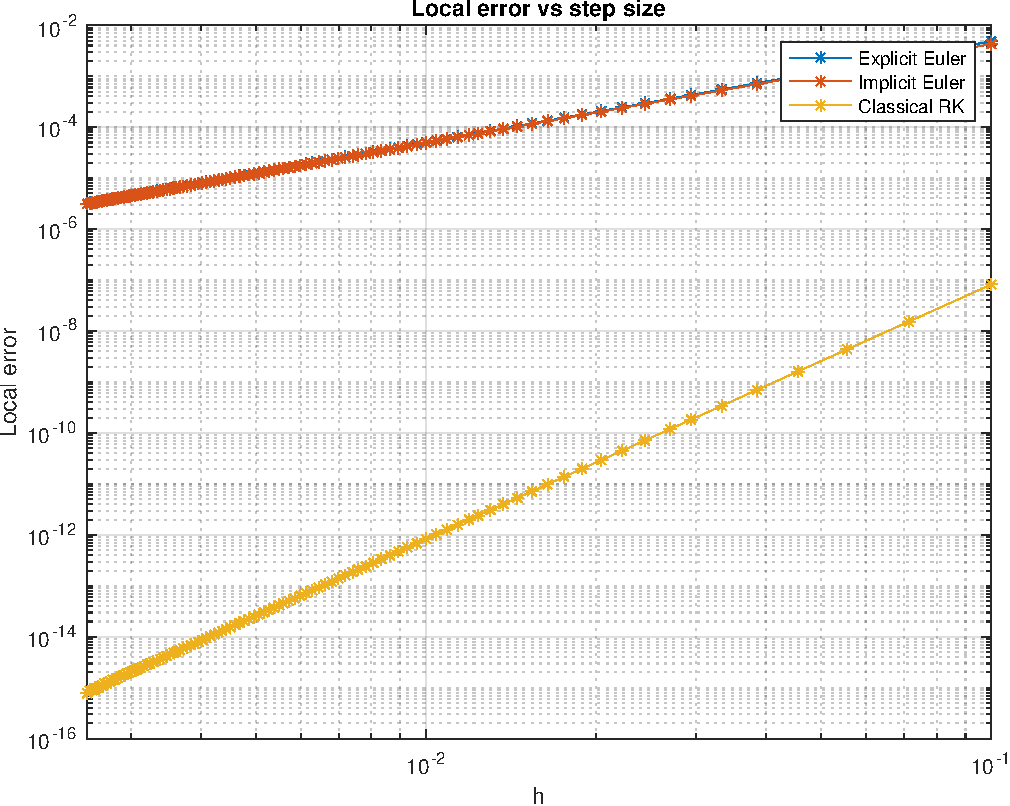
\includegraphics[width=0.7\textwidth]{plots/1_4.pdf}
    \caption{Caption}
    \label{fig:1_4}
\end{figure}



\subsection{Global error}

\subsection{Stability}
\clearpage
\section{Explicit ODE solver}
Considering the more general case of an \textit{Initial Value Problem}.
$$
\frac{d}{d t} x(t)= \dot{x}(t)=f(t, x(t), p), \quad x\left(t_{0}\right)=x_{0},
$$
where $x \in \mathbb{R}^{n_{x}}$ and $p \in \mathbb{R}^{n_{p}}$. In the following equations, the parameters p are implicit in $f(t, x(t)) = f(t, x(t), p)$.

\subsection{Explicit Euler}
The simplest numerical solver for this problem is the Explicit Euler which discretizes the continuous ODE by taking forward steps with the $\dot{x}(t_k) = f(t, x(t))$ in each iteration $k$ \cite{JrgensenScientificEquations}:

\begin{equation}
    x_{k+1}=x_{k}+\Delta t_k f\left(t_{k}, x_{k}\right)
\end{equation}

Where $\Delta t_k$ is the step size in iteration $k$. The method is analogous to taking the tangent in $x(t_k) = x_k$ and taking a $\Delta t_k$ step along the tangent:

\begin{equation}
\frac{x\left(t_{k+1}\right)-x\left(t_{k}\right)}{\Delta t_{k}} \approx \frac{d}{d t} x\left(t_{k}\right)=f\left(t_{k}, x\left(t_{k}\right)\right)
\end{equation}

Naturally a question arises on choosing an appropriate step size $\Delta t_k$. This gives rise to Explicit Euler with fixed step size

\begin{equation*}
    \Delta t_k = \Delta t = h \quad \forall_k
\end{equation*}

And with adaptive step size where $\Delta t_k$ can change in each iteration k. The ladder approach is discussed in further detail in Section 2.3.

\subsection{MATLAB implementation fixed step size}
See the following MATLAB implementation of the Explicit Euler with fixed step size (as described in Section 2.1), well-suited for non-stiff problems.

\begin{adjustwidth*}{0cm}{-0.4cm}
\begin{lstlisting}[frame=single, language=Matlab,caption=Explicit Euler (fixed step size), label=ExplicitEulerFixie]
function [T,X, fcount] = ExplicitEulerFixedStepSize(fun,t0,tN,N,x0,varargin)
% Compute step size and allocate memory
fcount = 0;
dt = (tN-t0)/N;
nx = size(x0,1);
X = zeros(nx,N+1);
T = zeros(1,N+1);

% Eulers Explicit Method
T(:,1) = t0;
X(:,1) = x0;
for k=1:N
    fcount = fcount +1;
    [f, Jac] = feval(fun,T(k),X(:,k),varargin{:});
    T(:,k+1) = T(:,k) + dt;
    X(:,k+1) = X(:,k) + f*dt;
end

% Form a nice table for the result
T=T';
X=X';
end
\end{lstlisting}
\end{adjustwidth*}

\subsection{MATLAB implementation adaptive step size}
\label{sec:ExplicitEulerAdaptive} \label{sec:stepdoubling}
See the following MATLAB implementation of the Explicit Euler with adaptive step size, well-suited for stiff and non-stiff problems. The embedded error estimation is based on \textit{stop doubling}, i.e. estimating the error of a full step from the more accurate two half-steps. Going in greater detail with the adaptive step size:

As mentioned, an Explicit Euler is taken with step size $\Delta {t_k}$ and then two half-steps is taken with step size $\Delta t_k$ and the \textit{error} of the Euler step is estimated as difference. I.e. 

\begin{equation}
\begin{aligned}
&x_{k+1}=x_{k}+\Delta t_k f\left(t_{k}, x_{k}\right) \\
&\hat{x}_{k+1 / 2}=x_{k}+\frac{\Delta t_k}{2} f\left(t_{k}, x_{k}\right) \\
&\hat{x}_{k+1}=\hat{x}_{k+1 / 2}+\frac{\Delta t_k}{2} f\left(t_{k}+\frac{\Delta t_k}{2}, \hat{x}_{k+1 / 2}\right) \\
&e_{k+1}=\hat{x}_{k+1}-x_{k+1}
\end{aligned}
\end{equation}

The r-coefficient is then calculated relative to chosen tolerances of the solution

\begin{equation}
r_{k+1}=\max _{i \in\{1, \ldots, n\}}\left\{\frac{\left|\left(e_{k+1}\right)_{i}\right|}{\max \left\{\text { abstol },\left|\left(x_{k+1}\right)_{i}\right| \text { reltol }\right\}}\right\}
\end{equation}

All cases where $r_{k+1} > 1$ is then rejected such that the error in each step $e_{k+1}$ is never great than the abstol nor the relative tolerence (reltol) times $(x_{k+1})_i$. 
\\
If $r_{k+1} > 1$ the step size is decreased until the criteria is fulfilled. Similarly, if $r_{k+1}$ is very low, i.e. the error is very low compared to our tolerances, the step size should be increased.
The step size $\Delta t_{k+1}$ is increased or decreased with the formula

\begin{equation}
\Delta t_{k+1}=\left(\frac{\varepsilon}{r_{k+1}}\right)^{1 / 2} \Delta t_{k}
\end{equation}

Where $\epsilon$ represents a target $r_{k+1}$ value. For robustness, a minimum and maximum scaling factor of the step size is chosen and denoted \textit{facmin} and \textit{facmax}. See the MATLAB implementation below for the Adaptive Explicit Euler. Note that $h = \Delta t_{k}$ has been used.

\begin{adjustwidth*}{0cm}{-0.4cm}
\begin{lstlisting}[frame=single, language=Matlab,caption=Explicit Euler (adaptive step size), label=ExplicitEulerFixie]
function [T,X,fcount,nreject] = ExplicitEulerAdaptiveStep(...
    fun,tspan,x0,h0,abstol,reltol,varargin)
epstol = 0.8;
facmin = 0.1;
facmax = 5.0;

t0 = tspan(1);
tf = tspan(2);
fcount = 0;
nreject = 0;

% Initial condtions
t = t0;
h = h0;
x = x0;

% Output
T = t;
X = x';
%% Main algorithm
while t < tf
    if (t + h >tf)
        h = tf-t;
    end
    fcount = fcount+1;
    f = feval(fun,t,x,varargin{:});

    AcceptStep = false;
    while ~AcceptStep
        %Take step of size h
        x1 = x+h*f;

        %Take step of size h/2
        hm = 0.5*h;
        tm = t + hm;
        xm = x + hm*f;
        fcount = fcount +1;
        fm = feval(fun,tm,xm,varargin{:});
        x1hat = xm + hm*fm;

        % Error estimation
        e = x1hat-x1; % Estimate of global error
        r = max(abs(e) ./ max(abstol,abs(x1hat).*reltol));

        AcceptStep = (r <= 1.0);
        if AcceptStep
            t = t+h;
            x = x1hat;

            T = [T;t];
            X = [X;x'];
        else
            nreject = nreject+1;
        end
        % Asymptotic step size controller
        h = max(facmin, min(sqrt(epstol/r), facmax))*h;
    end
end
\end{lstlisting}
\end{adjustwidth*}

\subsection{Van der Pol}
The Van der Pol oscillator problem is used extensively throughout this report to compare the different numerical solvers. It is defined as the 2nd order differential equation

\begin{equation}
\ddot{y}(t)=\mu\left(1-y(t)^{2}\right) \dot{y}(t)-y(t)
\end{equation}

Which can be rewritten to a 1st order differential equation \cite{JrgensenScientificEquationse}: 

\begin{equation}
\label{eq:vanderpol}
\begin{aligned}
&\dot{x}_{1}(t)=x_{2}(t) \\
&\dot{x}_{2}(t)=\mu\left(1-x_{1}(t)^{2}\right) x_{2}(t)-x_{1}(t)
\end{aligned}
\end{equation}

Where $y(t) = x_{1}(t)$.


\\\

The phase potraits as obtained by solving the Van der Pol problem (Eq. \ref{eq:vanderpol}) using the Adaptive Explicit Euler and Fixed (step size) Explicit Euler is seen in Figure \ref{fig:2_4a} and \ref{fig:2_4b}. The problem is solved for t = [0, 32] with $\mu = 3$ and $\mu =20$. Tolerances chosen are $reltol = abstol = \{10^{-2}, 10^{-4}, 10^{-6}\}$. Now a natural question arises, which fixed step sizes $h$ should be chosen for comparison with the adaptive method? The fixed step size $h$ was chosen to result in same number of steps as for the adaptive solution for comparison purposes.

\\
Clearly, for the stiff problem ($\mu = 20$) the fixed step size $h \approx 0.1$ is infeasible. The method is unstable and explodes towards $\infty$ (Figure \ref{fig:2_4a}). For the non-stiff problem ($\mu = 3$), the $h \approx 0.1$ is biased compared to the adaptive methods.
\\

When looking at tolerances of $\{10^{-4}, 10^{-6}\}$ seen in Figure \ref{fig:2_4b} the fixed step size is a lot more accurate, albeit a small bias in the non-stiff problem. For the stiff-problem $h=\frac{1612}{32}$ is very biased and only slightly biased for $h=\frac{14411}{32}$. There is no distinguishable difference between the Adaptive Euler and ode45/ode15s for tolerances $\geq 10^{-4}$.
\\

Note however that the Adaptive Explicit Euler uses a lot more function evaluations than the Fixed Explicit Euler. The choice is a trade-off between speed and accuracy.

\begin{figure}
    \centering
    \includegraphics[width=\textwidth]{plots/2_4main_02.pdf}
    \caption{Explicit Euler method tested on the Van der Pol problem. Both an adaptive step size strategy with tolerance = 0.01 and a fixed step size strategy fixed to equal number of steps is applied.}
    \label{fig:2_4a}
\end{figure}

\begin{figure}
    \centering
    \includegraphics[width=\textwidth]{plots/2_4main_04_06.pdf}
    \caption{Explicit Euler method tested on the Van der Pol problem. Both an adaptive step size strategy with tolerances $\in \{10^{-4}, 10^{-6}\}$ and a fixed step size strategy with an equivalent number of steps is applied.}
    \label{fig:2_4b}
\end{figure}

\subsection{Discussion of interface}
The methods have been implemented in a similar fashion to MATLAB's ode45 and ode15s for comparison purposes. For better comparison of fixed vs. adaptive step size, the implementation of the fixed step size was designed to be able to take a $N$ number of steps as input.
\clearpage
\section{Implicit ODE solver}
Considering again the \textit{Initial Value Problem}.
$$
\frac{d}{d t} x(t)= \dot{x}(t)=f(t, x(t), p), \quad x\left(t_{0}\right)=x_{0},
$$
where $x \in \mathbb{R}^{n_{x}}$ and $p \in \mathbb{R}^{n_{p}}$. In the following equations the parameters p are implicit in $f(t, x(t)) = f(t, x(t), p)$.

\subsection{Implicit Euler}
Whereas the Explicit Euler intuitively takes a discrete step forward with $\dot{x}_k$, one could say that the Implicit Euler intuitively takes a step \textit{backward} with $\dot{x}_{k+1} = f(t_{k+1}, x_{k+1})$ in each iteration \textit{k} \cite{JrgensenScientificEquationsb}:

\begin{equation}
    x_{k+1}=x_{k}+\Delta t_k f\left(t_{k+1}, x_{k+1}\right)
\end{equation}

Where $\Delta t_k$ is the step size in iteration \textit{k}. It discretises the continuous ODE in the same fashion as the Explicit Euler. The method is analogous to taking the tangent in $x(t_{k+1}) = x_{k+1}$ and taking a $\Delta t_k$ step along the tangent:

\begin{equation}
\frac{x\left(t_{k+1}\right)-x\left(t_{k}\right)}{\Delta t_{k}} \approx \frac{d}{d t} x\left(t_{k+1}\right)=f\left(t_{k+1}, x\left(t_{k+1}\right)\right)
\end{equation}

One natural hurdle arises: We don't know the $\dot{x}_{k+1} = f\left(t_{k+1}, x\left(t_{k+1}\right)\right) = f\left(t_{k+1}, x_{k+1}\right)$ because $x_{k+1}$ is unknown (it is the one we wish to calculate in iteration \textit{k}). Solution: Estimate it using \textit{Newton's method}.

\\\

\textbf{Newton's Method} \\
Newton's method finds the root of a residual function $R(x_{k+1})=0$ using a 1st order Taylor expansion at $x_{k+1}$:
\begin{equation}
    R(x_{k+1}) \approx R(x_k) + \frac{\partial R}{\partial x}\left(x_{k
    }\right)\left(x_{k+1} - x_{k}\right)
\end{equation}

Which can be solved as a linear system of equations \cite{JrgensenScientificEquationsb}. So by formulating the Implicit Euler problem as a residual function: 

\begin{equation}
R\left(x_{k+1}\right)=x_{k+1}-\Delta t f\left(t_{k+1}, x_{k+1}\right)-x_{k}=0
\end{equation}

One can implicitly estimate $x_{k+1}$ by minimising the residual function. In practice, one chooses a tolerance $\epsilon$ for criteria of convergence where $\|R(x)\|_{\infty} \leq \epsilon$ or if a maximum number of iterations has been reached. Using the linear systems formulation, the function is then minimised by Newton's Method by iterating over

$$
\begin{aligned}
&M \Delta x_{k+1}=R\left(x_{k+1}^{[l]}\right) \\
&x_{k+1}^{[l+1]}=x_{k+1}^{[l]}-\Delta x
\end{aligned}
$$

in each iteration \textit{l} where $M=\frac{\partial R}{\partial x}\left(x_{k+1}\right)$ [ibid.]. A decent initial guess at $l=0$ is the simple Explicit Euler step:

$$
x_{k+1}^{[0]}=x_{k}+\Delta t_k f\left(t_{k}, x_{k}\right)
$$

\\\

As with the Explicit Euler, a question arises on choosing an appropriate step size $\Delta t_k$. This gives rise to Implicit Euler with fixed step size:

\begin{equation*}
    \Delta t_k = \Delta t = h \quad \forall_k
\end{equation*}

or Implicit Euler with adaptive step size where $\Delta t_k$ changes in each iteration k. The ladder approach is discussed in further detail in Section 3.3.













\subsection{MATLAB implementation fixed step size}
See the following MATLAB implementation of the Implicit Euler with fixed step size (as described in Section 3.1), well-suited for non-stiff problems.

\begin{adjustwidth*}{0cm}{-0.4cm}
\begin{lstlisting}[frame=single, language=Matlab,caption=Implicit Euler (fixed step size), label=ImplicittEulerFixie]
function [T,X] = ImplicitEulerFixedStepSize(funJac,ta,tb,N,xa,varargin)
    % Compute step size and allocate memory
    dt = (tb-ta)/N;
    nx = size(xa,1);
    X = zeros(nx,N+1);
    T = zeros(1,N+1);

    tol = 1.0e-8;
    maxit = 100;
    % Eulers Implicit Method
    T(:,1) = ta;
    X(:,1) = xa;
    for k=1:N
        [f, J] = feval(funJac,T(k),X(:,k),varargin{:}); T(:,k+1) = T(:,k) + dt;
        xinit = X(:,k) + f*dt;
        X(:,k+1) = NewtonsMethodODE(funJac,...
            T(:,k), X(:,k), dt, xinit, tol, maxit, varargin{:});
    end
    % Form a nice table for the result
    T=T';
    X=X';
end
\end{lstlisting}
\end{adjustwidth*}

Which utilises Newton's Method:

\begin{adjustwidth*}{0cm}{-0.4cm}
\begin{lstlisting}[frame=single, language=Matlab,caption=Newton's Method, label=Newton]
function x = NewtonsMethodODE(FunJac, tk, xk, dt, xinit, tol, maxit, varargin)
    k=0;
    t=tk+dt;
    x = xinit;
    [f,J] = feval(FunJac,t,x,varargin{:});
    R=x-f*dt-xk;
    I = eye(length(xk));
    while( (k < maxit) & (norm(R,'inf') > tol) )
        k=k+1;
        dRdx=I-J*dt;
        dx = dRdx\R;
        x=x-dx;
        [f,J] = feval(FunJac,t,x,varargin{:});
        R=x-dt*f-xk;
    end
end
\end{lstlisting}
\end{adjustwidth*}















\subsection{MATLAB implementation adaptive step size}
See the following MATLAB implementation of the Implicit Euler with adaptive step size, well-suited for stiff and non-stiff problems. The embedded error estimation is based on \textit{stop doubling}, i.e. estimating the error of a full step from the more accurate two half-steps. This procedure has been explained in full detail in Section \ref{sec:ExplicitEulerAdaptive}. The Newton's Method implementation is the same as in Listing \ref{Newton}.

\begin{adjustwidth*}{0cm}{-0.4cm}
\begin{lstlisting}[frame=single, language=Matlab,caption=Implicit Euler (adaptive step size), label=ExplicitEulerFixie]
function [T,X,iter] = ImplicitEulerAdaptiveStep(...
    funJac,tspan,x0,h0,abstol,reltol,varargin)
epstol = 0.8;
facmin = 0.1;
facmax = 5.0;

t0 = tspan(1);
tf = tspan(2);

iter = 0;
% Initial condtions
t = t0;
h = h0; % = dt (step size - bliver modificeret)
x = x0;

% Output
T = t;
X = x';

% Newton syuff
tol = 1e-05;
maxit = 1000;

%% Main algorithm
while t < tf
    iter = iter +1;
    if (t + h >tf)
        h = tf-t;
    end
    f = feval(funJac,t,x,varargin{:});
    AcceptStep = false;
    while ~AcceptStep
        %Take step of size h
        xinit = x + h*f; % Gæt på x+1
        x1 = NewtonsMethodODE(funJac, t, x, h, xinit, tol, maxit, varargin{:});

        %Take step of size h/2
        hm = 0.5*h;
        xinitm = x + hm*f;
        tm = t + hm;

        xm = NewtonsMethodODE(funJac, tm, x, hm, xinitm, tol, maxit, varargin{:});
        
        xinitm2 = x + 2*hm*f ; % = xinit (og derfor redundant)
        x1hat = NewtonsMethodODE(funJac, tm, xm, hm, xinitm2, tol, maxit, varargin{:});

        % Error estimation
        e = x1hat-x1; % Estimate of global error
        r = max(abs(e) ./ max(abstol,abs(x1hat).*reltol));

        AcceptStep = (r <= 1.0);
        if AcceptStep
            t = t+h;
            x = x1hat;

            T = [T;t];
            X = [X;x'];
        end
        % Asymptotic step size controller
        h = max(facmin, min(sqrt(epstol/r), facmax))*h;
    end
end
\end{lstlisting}
\end{adjustwidth*}










\subsection{Van der Pol}
The phase potraits as obtained by solving the Van der Pol problem (Eq. \ref{eq:vanderpol}) using the Adaptive Implicit Euler and Fixed (step size) Implicit Euler is seen in Figure \ref{fig:3_4a} and \ref{fig:3_4b}. The problem is solved for t = [0, 32] with $\mu = 3$ and $\mu =20$. Tolerances chosen are $reltol = abstol = \{10^{-2}, 10^{-4}, 10^{-6}\}$. Again, the fixed step sizes $h$ has been chosen to result in same number of steps as for the adaptive solution for comparison purposes.
\\
In Figure \ref{fig:3_4a} and \ref{fig:3_4b} it is clear that the fixed step size is infeasible for the stiff problem ($\mu = 20$) until \textit{h} becomes very small h=$10^{-5.5}$ where it assimilates the behaviour of ode45 and ode15s. Remember that for \textit{h} becoming infinitesimally small the approximation becomes exact, so even for stiff problems a fixed step size Euler method can solve the problem accurate (but inefficient) by choosing an extremely small \textit{h}.\\
For the non-stiff problem ($\mu = 3$) the Fixed Implicit Euler is not as crude of an approximation. Note however how the ode45 and ode15s requires much fewer (albeit more expensive) steps than the corresponding Adaptive Implicit Euler. \\
Interestingly, it takes much fewer step to guarantee the specified tolerances in the stiff problem than for the non-stiff problem. 

\\
Note on both plots how the Implicit Euler is biased inwards in the phase portrait whereas the Explicit Euler was biased outward. This is due to the very nature of the backward vs forward step of the two methods.

\\



\begin{figure}
    \centering
    \includegraphics[width=\textwidth]{plots/3_4main.pdf}
    \caption{Implicit Euler method tested on the Van der Pol problem. Both an adaptive step size strategy with tolerances $\in \{1e-02, 1e-04, 1e-06\}$ and a fixed step size strategy fixed to an equal number of steps is applied.}
    \label{fig:3_4a}
\end{figure}

\begin{figure}
    \centering
    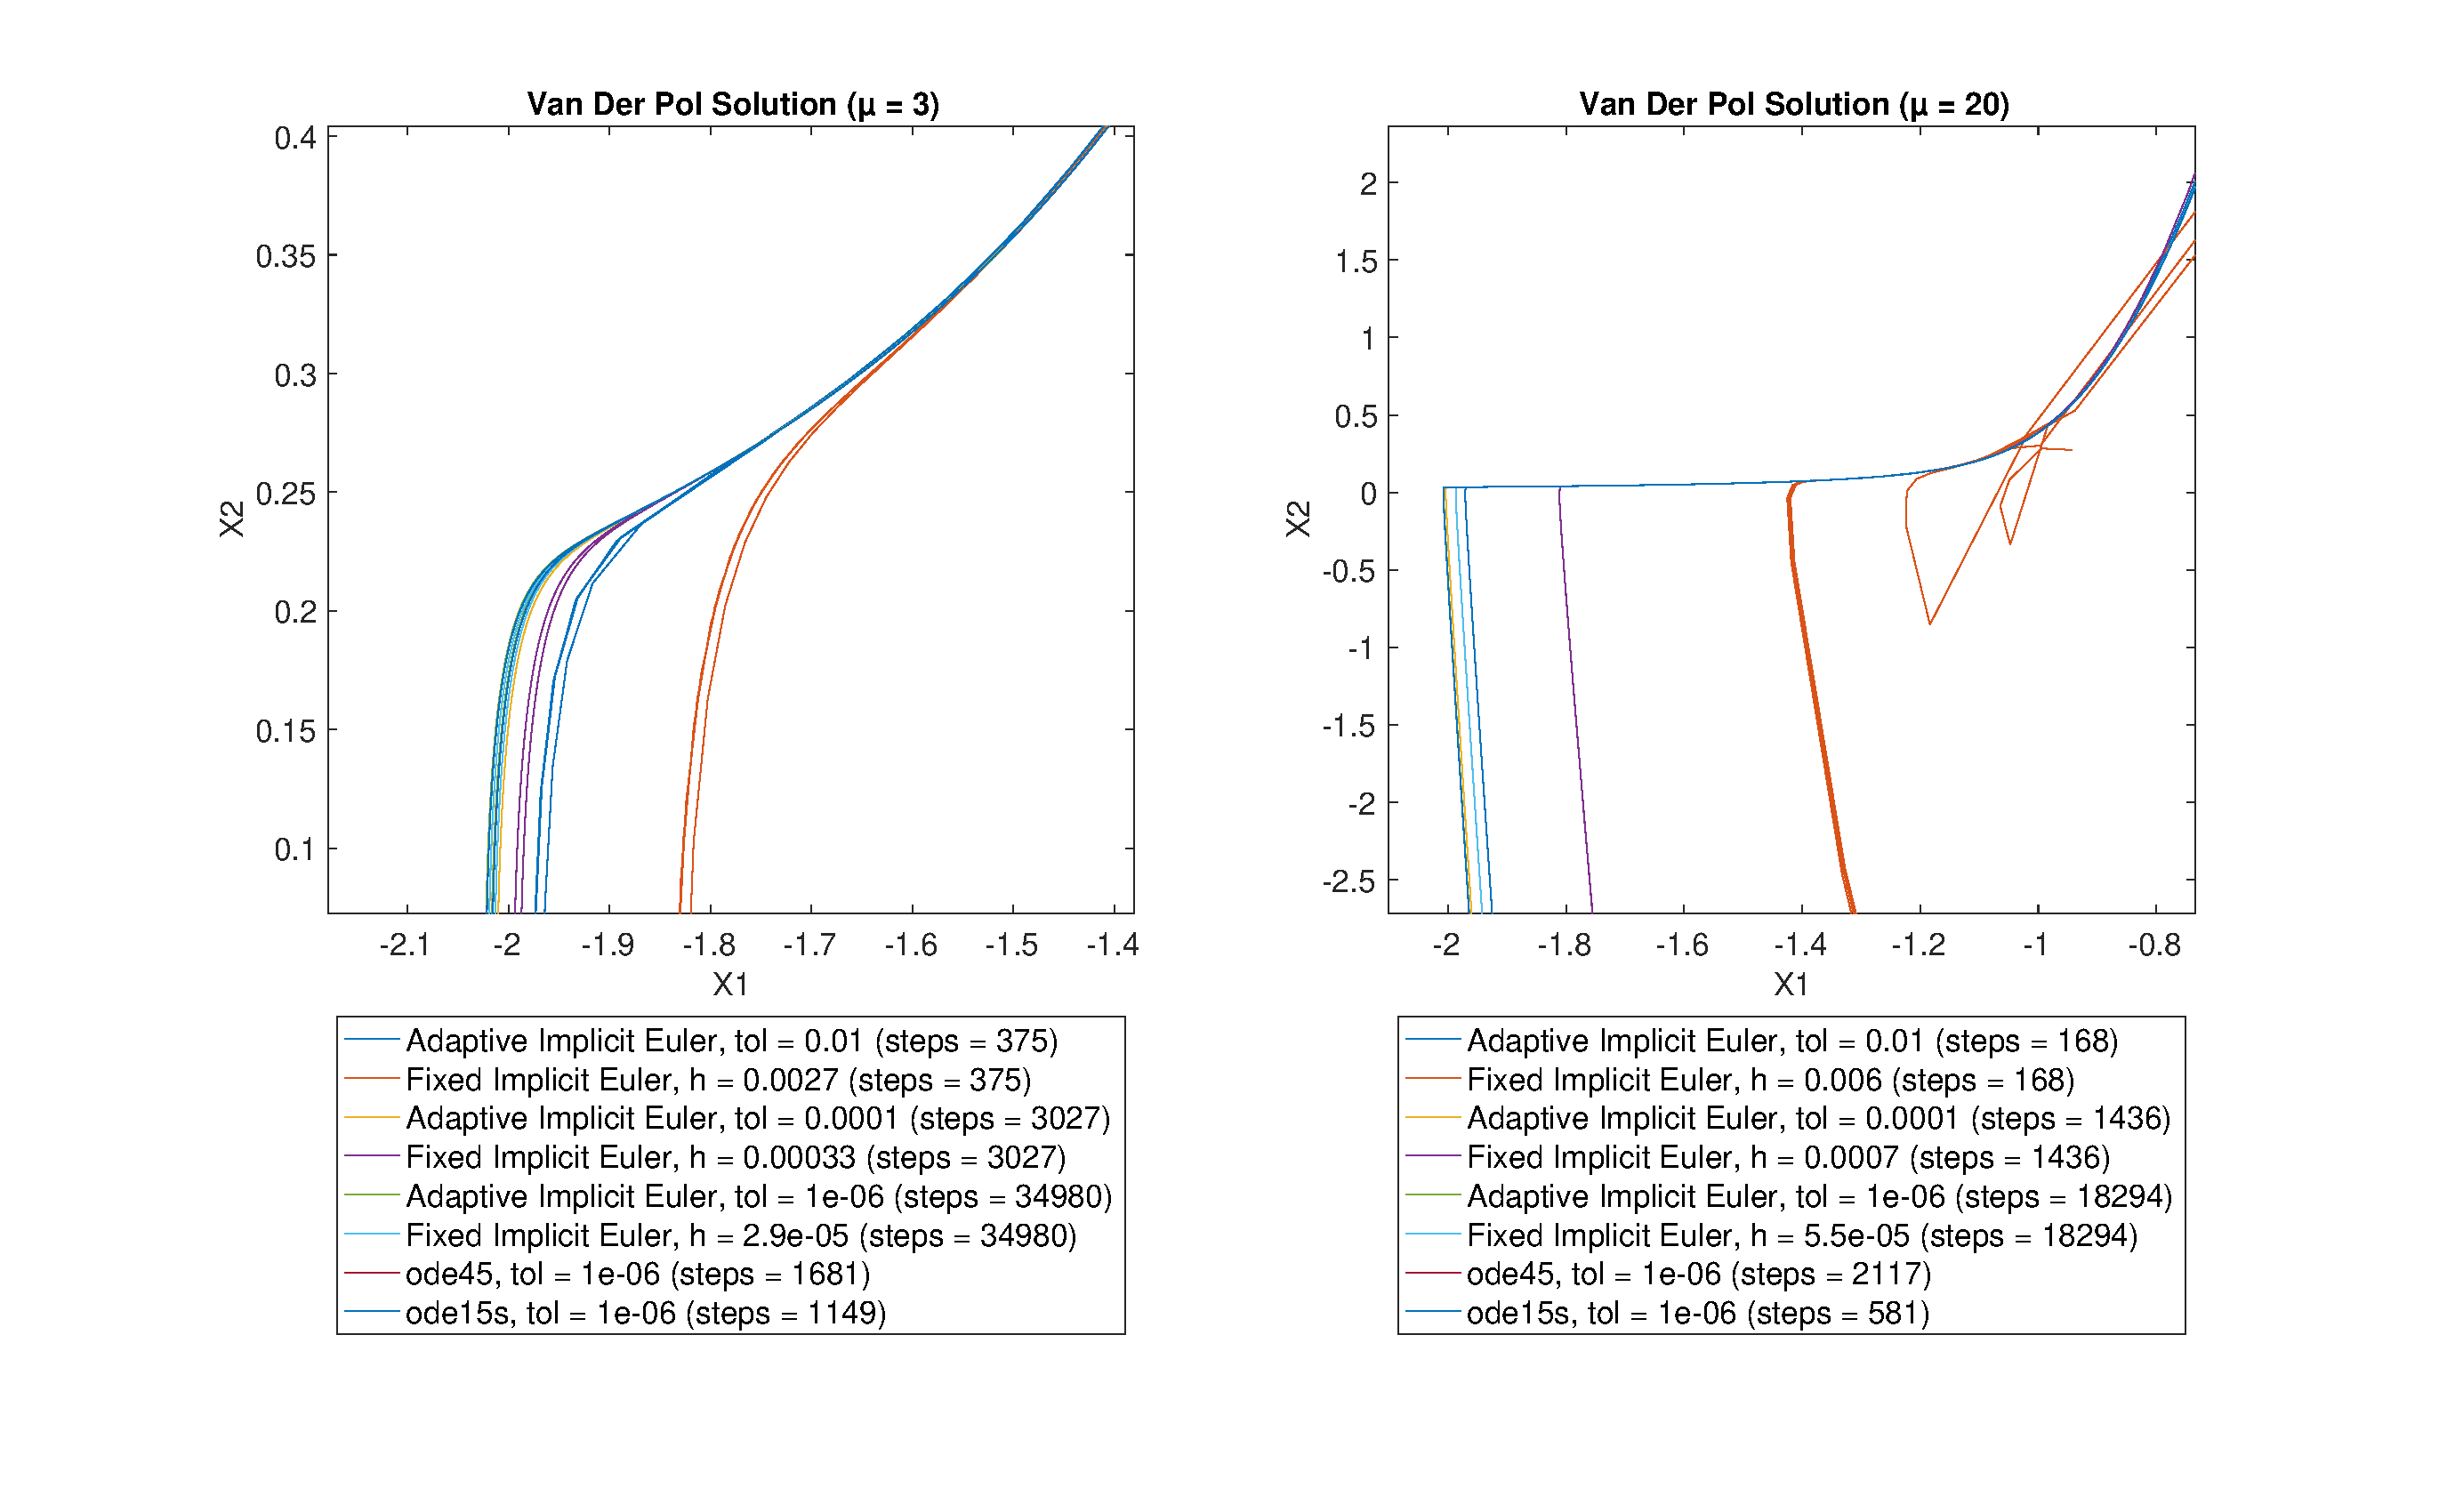
\includegraphics[width=\textwidth]{plots/3_4main_zoom.eps}
    \caption{Zoom-in of the Implicit Euler method tested on the Van der Pol problem. Both an adaptive step size strategy with tolerance = 0.01 and a fixed step size strategy fixed to equal number of steps is applied.}
    \label{fig:3_4b}
\end{figure}




\subsection{Discussion of interface}
In this sections we have seen the Implicit Euler method, where the calculation of $x_{k+1}$ is done implicitly. We have seen how it still takes the Implicit Euler method a lot more steps to ensure a specific accuracy than the ode45 and ode15s. This calls for more sophisticated methods which will begin with Runge-Kutta methods in Section 5.
\\
The Implicit Euler methods have been implemented in a similar fashion to MATLAB's ode45 and ode15s for comparison purposes. For better comparison of fixed vs. adaptive step size, the implementation of the fixed step size was designed to take a $N$ number of steps as input.


\clearpage
\section{Solvers for SDEs}
Considering now the stochastic differential equation (SDE)
$$
d x(t)=f\left(t, x(t), p_{f}\right) d t+g\left(t, x(t), p_{g}\right) d \omega(t) \quad d \omega(t) \sim N_{i i d}(0, I \Delta t)
$$

where $x \in \mathbb{R}^{n_{x}}$ and $\omega$ is a multivariate stochastic variable following a Wiener Process. The first term \textit{f()} is commonly referred to as the \textit{drift term} and the ladder term \textit{g()} is commonly referred to as the \textit{diffusion term}. The ODE is a particular case of an SDE where $g() = 0$. If the diffusion $g()$ does not change for different values of $x(t)$ the diffusion is said to be \textit{state independent} and said to be \textit{state dependent} otherwise.

\subsection{Wiener Process}
The Wiener Process is a stochastic process (a sequence of stochastic variables) realised from identical and independent Gaussian distributions with 0 mean and variance increasing with time \textit{dt}. It therefore models continuous perturbations allowing for greater variation when more time has passed. Using the reparametrization trick one can pull out the variance and use the standard Gaussian. It is implemented in MATLAB as follows:

\begin{adjustwidth*}{0cm}{-0.4cm}
\begin{lstlisting}[frame=single, language=Matlab,caption=Wiener Process, label=LittleWiener]
function [W,Tw,dW] = StdWienerProcess(T,N,nW,Ns,seed)
if nargin == 4
    rng(seed);
end
dt = T/N; % Fixed step size
dW = sqrt(dt)*randn(nW,N,Ns);
W = [zeros(nW,1,Ns) cumsum(dW,2)];
Tw = 0:dt:T;
\end{lstlisting}
\end{adjustwidth*}

\subsection{Explicit-Explicit (Euler-Maruyama)}
An SDE solver has to address both the drift term and the diffusion term. By linearity of integration the integral can be split into two integrals

\begin{equation}
\boldsymbol{x}\left(t_{k+1}\right)-\boldsymbol{x}\left(t_{k}\right)=\int_{t_{k}}^{t_{k+1}} f(\boldsymbol{x}(t)) d t+\int_{t_{k}}^{t_{k+1}} g(\boldsymbol{x}(t)) d \boldsymbol{\omega}(t)
\end{equation}

The drift term can be solved by a Riemann integral for which we have numerous approximation methods normally associated with ODEs. The diffusion term however requires an Itô integral \cite{JrgensenScientificEquationsd}. "Explicit-Explicit" refers to solving the drift term with an explicit method and the diffusion term with an explicit method. We will use the Euler-Maruyama for approximating the solution to the SDE:

\begin{equation}
\boldsymbol{x}_{k+1}-\boldsymbol{x}_{k}=f\left(\boldsymbol{x}_{k}\right) \Delta t_{k}+g\left(\boldsymbol{x}_{k}\right) \Delta \boldsymbol{w}_{k}
\end{equation}

Where we will use a fixed step size $\Delta t_k = \Delta t$. Note how the SDE is discretized as usual. It is based on a forward step $f\left(\boldsymbol{x}_{k}\right)$ for the drift and a forward step $g\left(\boldsymbol{x}_{k}\right)$ for the diffusion, i.e. Explicit-Explicit. The MATLAB implementation is found below.

\begin{adjustwidth*}{0cm}{-0.4cm}
\begin{lstlisting}[frame=single, language=Matlab,caption=Euler-Maruyama, label=hnrkmdsen]
function X = SDEsolverExplicitExplicit(ffun,gfun,T,x0,W,varargin)
N = length(T);
nx = length(x0);
X = zeros(nx,N);

X(:,1) = x0;
for k=1:N-1
    f = feval(ffun,T(k),X(:,k),varargin{:});
    g = feval(gfun,T(k),X(:,k),varargin{:});
    dt = T(k+1)-T(k); % Allow for varying step size
    dW = W(:,k+1)-W(:,k);
    psi = X(:,k) + g*dW; % The diffusion/pertubation 
    X(:,k+1) = psi + f*dt; % Add the drift
end
\end{lstlisting}
\end{adjustwidth*}

\subsection{Implicit-Explicit}
Now the drift term can also be solved by an Implicit Euler method as shown in Section 3. The approximation to the SDE is then

\begin{equation}
\boldsymbol{x}_{k+1}=\boldsymbol{x}_{k}+f\left(\boldsymbol{x}_{k+1}\right) \Delta t_{k}+g\left(\boldsymbol{x}_{k}\right) \Delta \boldsymbol{w}_{k}
\end{equation}

Where we will use a fixed step size $\Delta t_k = \Delta t$. Note how it is based on $f\left(\boldsymbol{x}_{k+1}\right)$ for the drift, where $x_{k+1}$ is unknown and calculated implicitly. The step for the diffusion is an explicit forward step $g\left(\boldsymbol{x}_{k}\right)$ for the diffusion. In other words, the method is an Implicit-Explicit method. The MATLAB implementation is found below.

\begin{adjustwidth*}{0cm}{-0.4cm}
\begin{lstlisting}[frame=single, language=Matlab,caption=Implicit-Explicit, label=implicitexplicit]
function X=SDEsolverImplicitExplicit(ffun,gfun,T,x0,W,tol,varargin)
maxit = 100;

N = length(T);
nx = length(x0);
X = zeros(nx,N);

X(:,1) = x0;
k=1;
[f,~] = feval(ffun,T(k),X(:,k),varargin{:});
for k=1:N-1
    g = feval(gfun,T(k),X(:,k),varargin{:});
    dt = T(k+1)-T(k);
    dW = W(:,k+1)-W(:,k);
    psi = X(:,k) + g*dW;
    xinit = psi + f*dt;
    [X(:,k+1),f,~] = SDENewtonSolver(...
            ffun,...
            T(:,k+1),dt,psi,xinit,...
            tol,maxit,varargin{:});
end
\end{lstlisting}
\end{adjustwidth*}

As with the Implicit Euler in Section 3, it is based on Newton's method for finding a root of the residual function by iteratively taking steps along the Jacobian evaluated in the current iteration. The implementation is seen in Listing \ref{newtonsde}.

\begin{adjustwidth*}{0cm}{-0.4cm}
\begin{lstlisting}[frame=single, language=Matlab,caption=Newton's Method for SDEs, label=newtonsde]
function [x,f,J] = SDENewtonSolver(ffun,t,dt,psi,xinit,tol,maxit,varargin)
I = eye(length(xinit));
x = xinit;
[f,J] = feval(ffun,t,x,varargin{:});
R = x - f*dt - psi;

it=1;
while( (norm(R,'inf') > tol) && (it <= maxit) )
    dRdx = I - J*dt;
    mdx = dRdx\R;
    x = x - mdx;
    [f,J] = feval(ffun,t,x,varargin{:});
    R = x - f*dt - psi;
    it = it+1;
end
\end{lstlisting}
\end{adjustwidth*}


\subsection{Description of implementations}
Implementations and methods has already been described and code included under the relevant methods in Section 4.2 and 4.3.

\subsection{Van der Pol}
In this section the above listed MATLAB implementations are tested on the Van der Pol problem. Until now we have only modelled a deterministic drift. The Van der Pol problem is now extended with a diffusion term. Two different diffusion functions will be tested, a state independent and state dependent respectively:

\begin{align*}
    & g(t, \boldsymbol{x}(t), \sigma) = [0, \sigma]^T \quad (1) \\
    & g(t, \boldsymbol{x}(t), \sigma) = [0, \sigma (1 + x_1(t)^2)]^T \quad (2)
\end{align*}

Resulting in SDE version (1) of the Van der Pol problem:

\begin{equation}
\label{sde1}
\begin{aligned}
d x_{1}(t) &=x_{2}(t) d t \\
d x_{2}(t) &=\left[\mu\left(1-x_{1}(t)^{2}\right) x_{2}(t)-x_{1}(t)\right] d t+\sigma d \omega(t)
\end{aligned}
\end{equation}

And SDE version (2) of the Van der Pol problem:

\begin{equation}
\label{sde2}
\begin{aligned}
&d x_{1}(t)=x_{2}(t) d t \\
&d x_{2}(t)=\left[\mu\left(1-x_{1}(t)^{2}\right) x_{2}(t)-x_{1}(t)\right] d t+\sigma\left(1+x_{1}(t)^{2}\right) d \omega(t)
\end{aligned}
\end{equation}

And fixed step size of $\Delta t = h = 0.001$ is used.







\\\

\textbf{Version (1) - state independent diffusion}\\
In this section, equation (\ref{sde1}) is solved with the two mentioned solvers with \\
\begin{center}
    $\mu \in \{3, 20\}$ and $\sigma \in \{0.1, 2.0\}$
\end{center}
as seen in Figure \ref{fig:4b} and \ref{fig:4a}. For comparison, the exact same realizations from the Wiener Process is used for the two solvers. There is a high impact from $\sigma$ but for comparing Explicit-Explicit vs Implicit-Explicit there is only a slight visible difference between the two when $\mu = 20$ in Figure \ref{fig:4a}.


\begin{figure}[H]
    \centering
    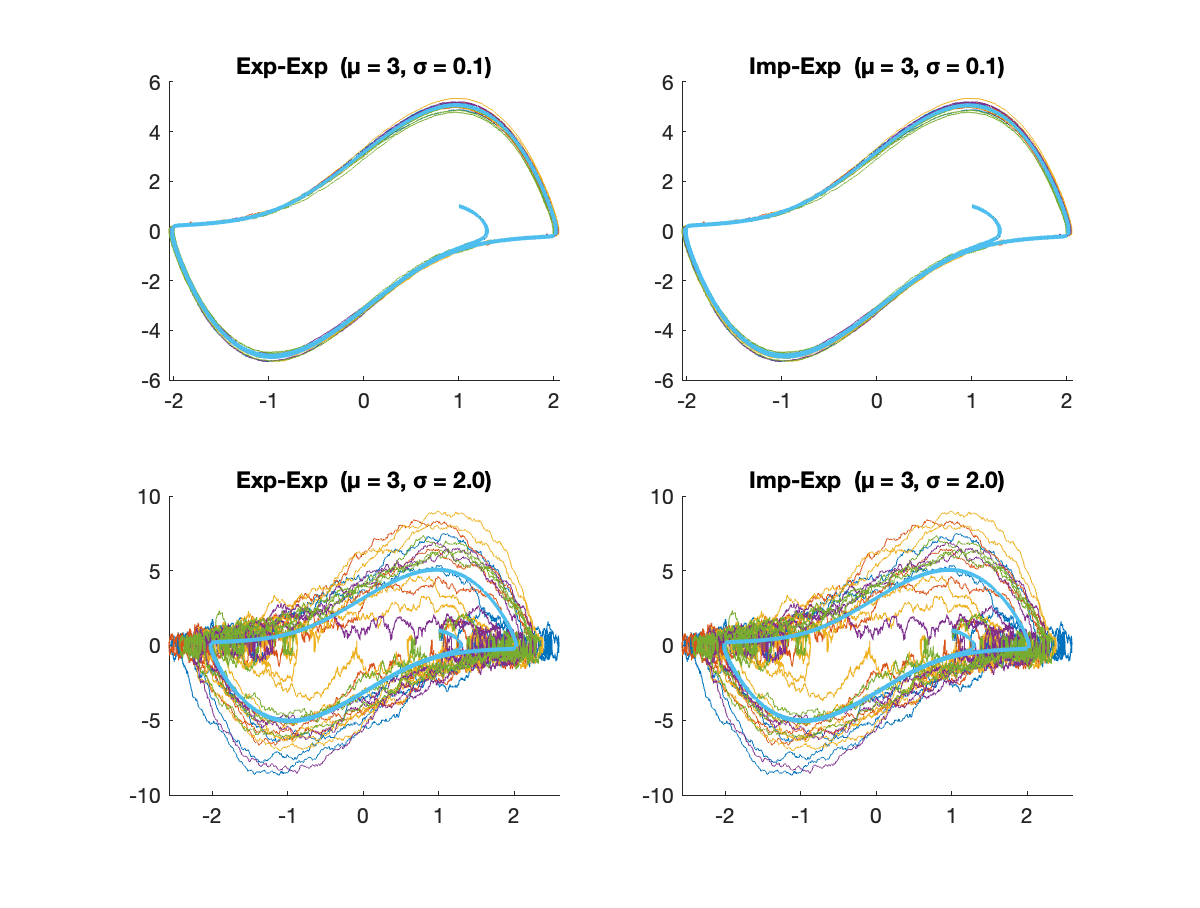
\includegraphics[width=\textwidth]{plots/4b.eps}
    \caption{Solution of the state independent diffusion Van der Pol SDE with varying $\sigma$.}
    \label{fig:4b}
\end{figure}

\begin{figure}[htb]
    \centering
    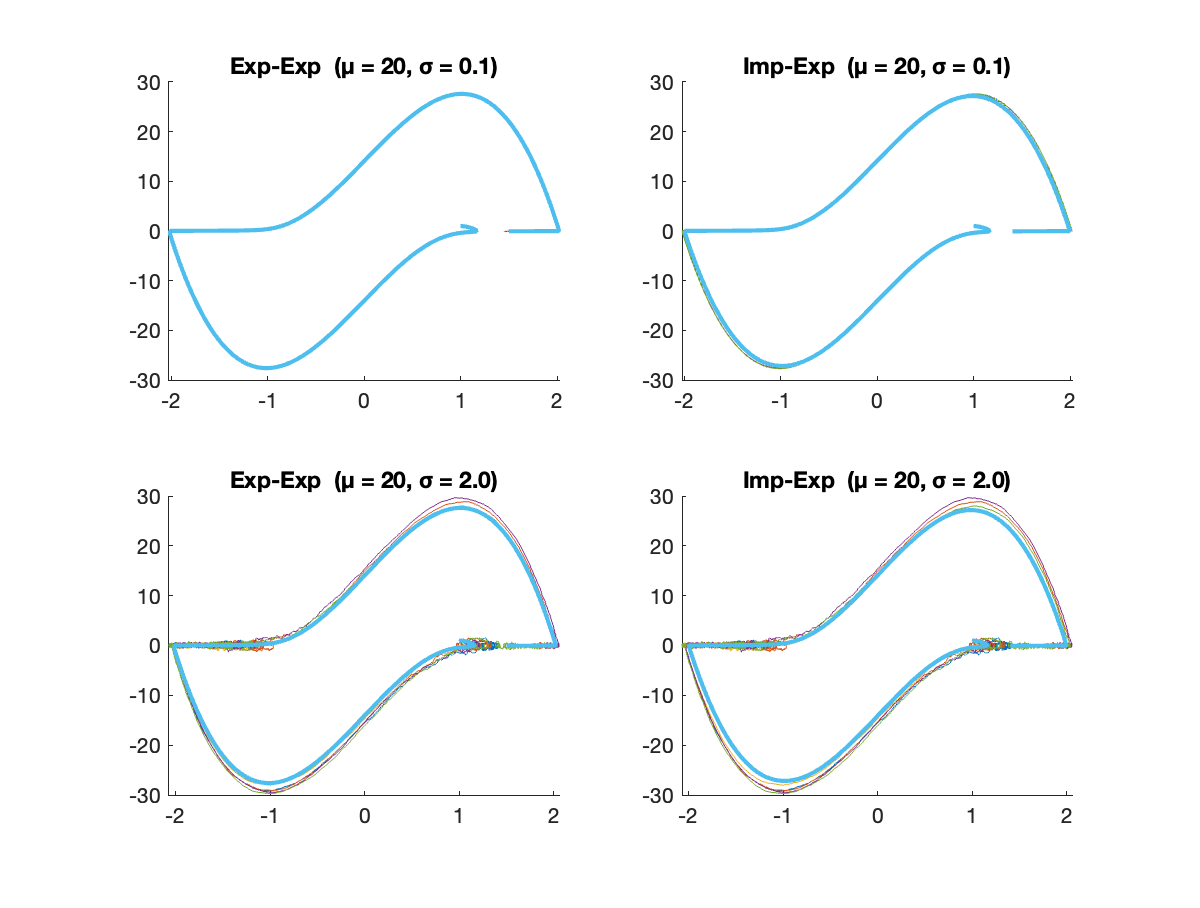
\includegraphics[width=\textwidth]{plots/4a.eps}
    \caption{Solution of the state independent diffusion Van der Pol SDE with varying $\sigma$.}
    \label{fig:4a}
\end{figure}


\\\

\textbf{Version (2) - state independent diffusion}\\
In this section, equation (\ref{sde2}) is solved with the two mentioned solvers with\\
\begin{center}
$\mu \in \{3, 20\}$ and $\sigma \in \{0.1, 2.0\}$     
\end{center}
as seen in Figure \ref{fig:4d} and \ref{fig:4c}. Again, the exact same realizations from the Wiener Process is used for the two solvers. There is a very high impact from $\sigma$, which for higher values makes the solution completely unstable. Interestingly, it is seen in Figure \ref{fig:4c} that the pertubations mainly effect the stiff regions of the ODE. For comparing Explicit-Explicit vs Implicit-Explicit one can only glimpse a small difference between the upper two plots in Figure \ref{fig:4c}. For this small of a step size (h = 0.001) the two approximations are almost identical.

\begin{figure}[htb]
    \centering
    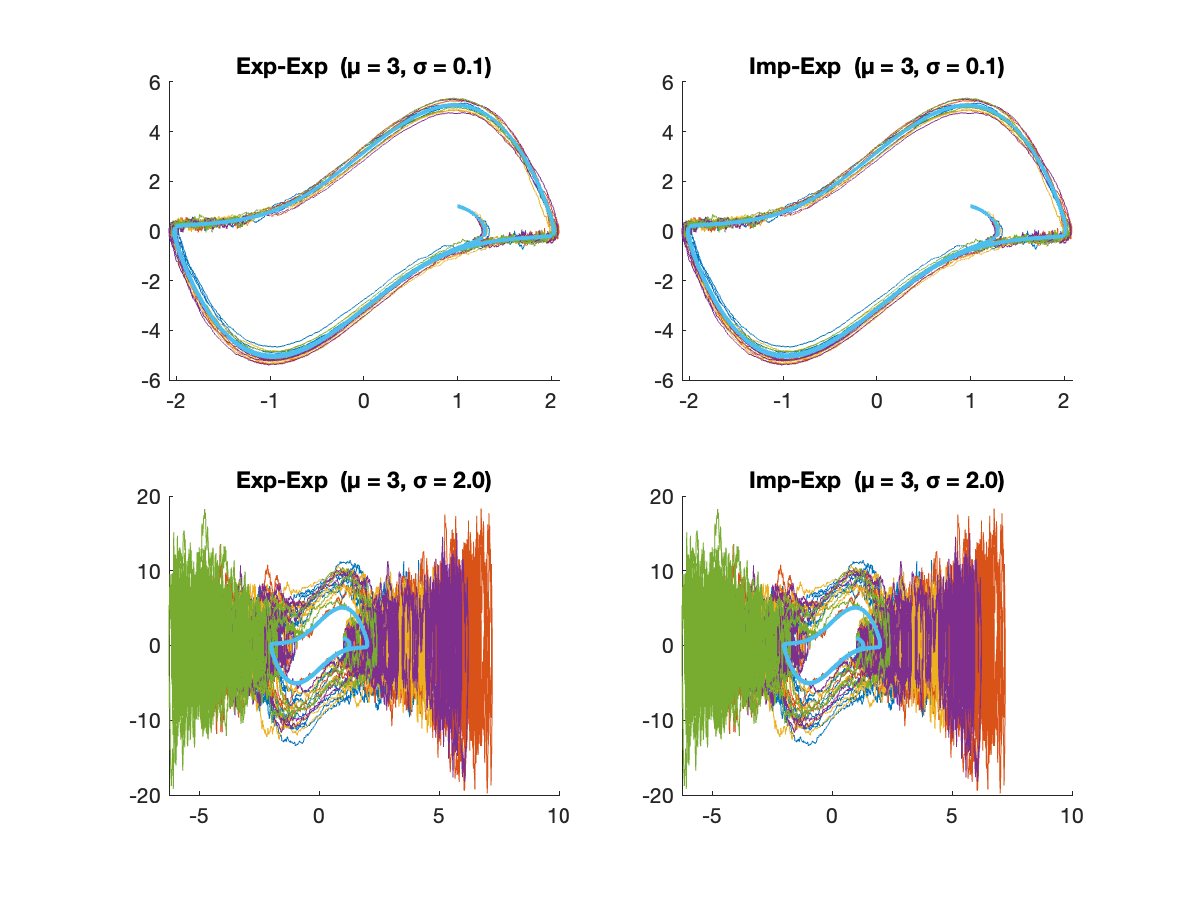
\includegraphics[width=\textwidth]{plots/4d.eps}
    \caption{Solution of the state dependent diffusion Van der Pol SDE with varying $\sigma$.}
    \label{fig:4d}
\end{figure}


\begin{figure}[htb]
    \centering
    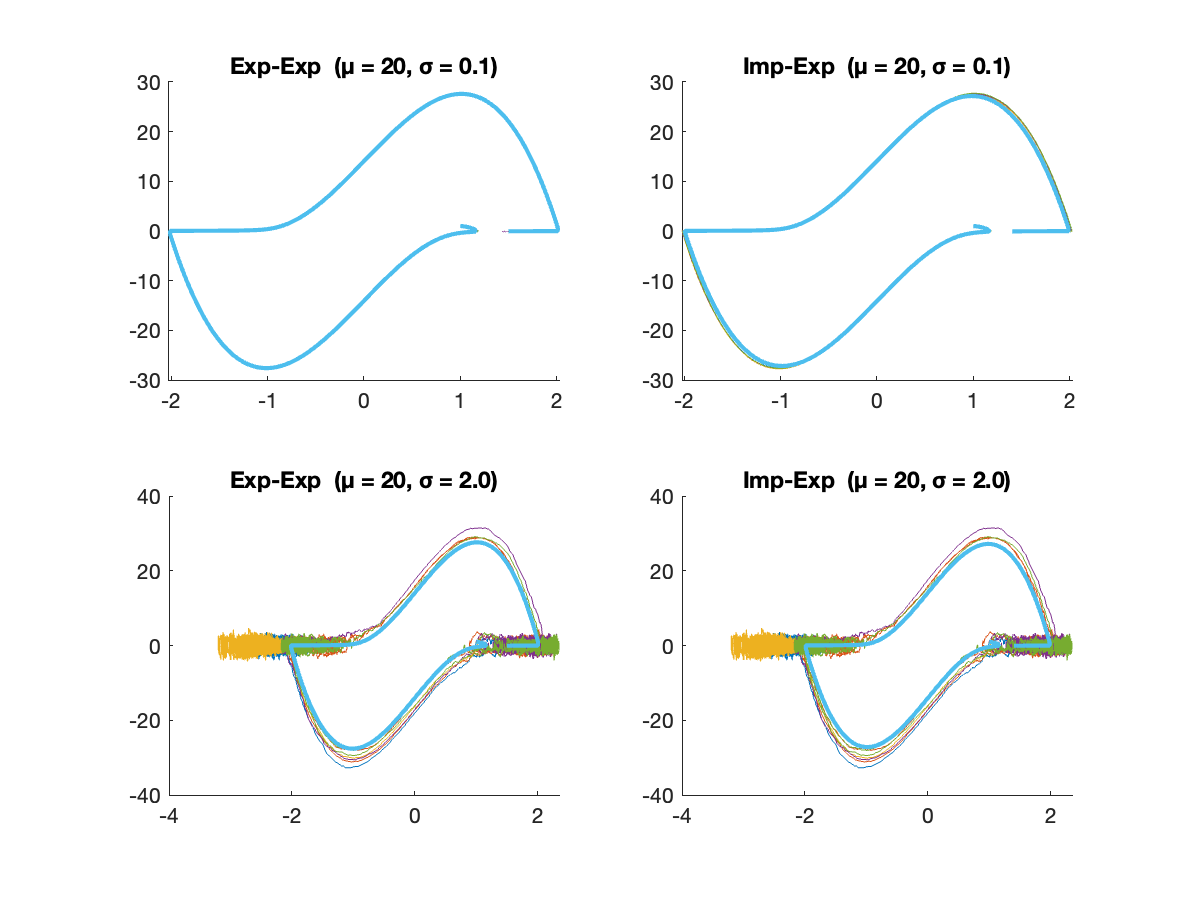
\includegraphics[width=\textwidth]{plots/4c.eps}
    \caption{Solution of the state dependent diffusion Van der Pol SDE with varying $\sigma$.}
    \label{fig:4c}
\end{figure}

\\\

In conclusion, two different numerical solvers has been proposed and shown feasible for solving stochastic differential equations.
\clearpage



\section{ESDIRK23}
Now another particular case of a Runge-Kutta method is the Explicit Singly Diagonal Implicit Runge-Kutta of 2nd order and 3rd order error estimation (ESDIRK23). The problem with Explicit Runge-Kutta methods is their relative small stability regions. None of them are A-stable and therefore neither L-stable. By spending the degrees of freedom cleverly as we will see, A-stability and L-stability can be achieved.

\\\

ESDIRK is family of methods sharing the same Butcher's Tableau, here illustrated for ESDIRK23 methods:

\begin{table}[H]
    \centering
\begin{tabular}{c|ccc}
0 & 0 & & \\
$c_{2}$ & $a_{21}$ & $\gamma$ & \\
1 & $b_{1}$ & $b_{2}$ & $\gamma$ \\
\hline$x_{n+1}$ & $b_{1}$ & $b_{2}$ & $\gamma$ \\
$\hat{x}_{n+1}$ & $\hat{b}_{1}$ & $\hat{b}_{2}$ & $\hat{b}_{3}$ \\
\hline$e_{n+1}$ & $d_{1}$ & $d_{2}$ & $d_{3}$
\end{tabular}
    \caption{Butcher's Tableau for the general ESDIRK23.}
    \label{tab:ESDIRK23general}
\end{table}

From $a_{1,1} = 0$ it follows that the method starts with an explicit step (saved from the previous iteration), i.e. $T_{1}=t_{n}, \quad X_{1}=x_{n}, \quad f_1 = f(t_n, x_n)$. Now the following two steps are implicit since the calculation of $X_2$ and $X_3$ \textit{depends} on $X_2$ and $X_3$ respectively. Note how they mutually share the same coefficient $\gamma$ making the method \textit{Singly Diagonal}. So how is $X_2$ and $X_3$ calculated implicitly? Using the Runge-Kutta equations \ref{eq:RKgeneral1} and \ref{eq:RKgeneral2} and using Newton's Method as explained in Section 3, we must solve

\begin{equation}
R\left(X_{2}\right)=X_{2}-h \gamma f\left(T_{2}, X_{2}\right)-x_{n}+h a_{21} f_{1}=0
\end{equation}
and
\begin{equation}
R\left(X_{3}\right)=X_{3}-h \gamma f\left(T_{3}, X_{3}\right)-x_{n}+h a_{31} f_{1}+h_{32} f_{2}=0
\end{equation}

Where $f_i = f(T_i, X_i)$. Note that since $c_3 = 1$, the 3rd stage corresponds to the full step $T_{3}=t_{n}+c_{3} h$ and therefore $x_{n+1} = X_3$. 



\subsection{Deriving ESDIRK23}
Now the question arises; What should the parameters be? By using the consistency condition 
\begin{equation}
C e=A e
\end{equation}

and order conditions (of order \textit{p)}

\begin{equation}
\Phi(\tau)=\frac{1}{\gamma(\tau)} \quad \forall r(\tau) \leq p
\end{equation}

and the table for the Taylor expansion terms \cite{JrgensenRunge-KuttaControl}:

\begin{equation}
\begin{array}{lcccccccc}
\hline \tau & \tau_{1} & \tau_{2} & \tau_{3} & \tau_{4} & \tau_{5} & \tau_{6} & \tau_{7} & \tau_{8} \\
r(\tau) & 1 & 2 & 3 & 3 & 4 & 4 & 4 & 4 \\
\sigma(\tau) & 1 & 1 & 2 & 1 & 6 & 1 & 2 & 1 \\
\gamma(\tau) & 1 & 2 & 3 & 6 & 4 & 8 & 12 & 24 \\
\Lambda(\tau) & I & C & C^{2} & A C & C^{3} & C A C & A C^{2} & A^{2} C \\
\Phi(\tau) & b^{\prime} e & b^{\prime} C e & b^{\prime} C^{2} e & b^{\prime} A C e & b^{\prime} C^{3} e & b^{\prime} C A C e & b^{\prime} A C^{2} e & b^{\prime} A^{2} C e \\
\Psi(\tau) & e & C e & C^{2} e & A C e & C^{3} e & C A C e & A C^{2} e & A^{2} C e \\
F(\tau) & f & f^{\prime} f & f^{\prime \prime}(f, f) & f^{\prime} f^{\prime} f & f^{\prime \prime \prime}(f, f, f) & f^{\prime \prime}\left(f, f^{\prime} f\right) & f^{\prime} f^{\prime \prime}(f, f) & f^{\prime} f^{\prime} f^{\prime} f \\
\hline
\end{array}
\caption{Functions on Rooted Trees.}
\end{equation}

We derive for the advancing method of order p=2:
\begin{align*}
    & b^T e = \frac{1}{1} \\
    & b^T C e = \frac{1}{2}
\end{align*}

And for the embedded method of order p=3:
\begin{align*}
    & \hat{b}^T e = \frac{1}{1} \\
    & \hat{b}^T C e = \frac{1}{2} \\
    & \hat{b}^T C^2 e = \frac{1}{3} \\
    & \hat{b}^T A C e = \frac{1}{6}
\end{align*}

Solving these equations there is still 1 degrees of freedom left. So choosing $\gamma=1-\frac{1}{\sqrt{2}}$ (see the attached Maple-sheet for details) we arrive at a well-defined ESDIRK23 which (by subtitution of coefficients) has the following Butcher's Tableau:

\begin{table}[H]
\centering
\begin{tabular}{c|ccc}
0 & 0 & 0 & 0 \\
$2-\sqrt{2}$ & $\frac{2-\sqrt{2}}{2}$  & $\frac{2-\sqrt{2}}{2}$ & 0 \\
$1$ & $\frac{\sqrt{2}}{4}$ & $\frac{\sqrt{2}}{4}$ & $\frac{2-\sqrt{2}}{2}$ \\ \hline
$x_{n+1}$ & $\frac{\sqrt{2}}{4}$ & $\frac{\sqrt{2}}{4}$ & $\frac{2-\sqrt{2}}{2}$ \\
$\hat{x}_{n+1}$ & $\frac{-\sqrt{2}+4}{12}$ & $\frac{3\sqrt{2}+4}{12}$ & $\frac{-\sqrt{2}+2}{6} $ \\ \hline
$e_{n+1}$ & $\frac{\sqrt{2}-1}{3}$ & $-\frac{1}{3}$ & $\frac{2-\sqrt{2}}{3}$
\end{tabular}
\caption{Butcher's Tableau of the derived ESDIRK23.}
\end{table}


Now as we shall see in the next section the choice of $\gamma$ was not a pure random one.

\subsection{Stability}
One can show as done in \cite{JrgensenRunge-KuttaControl} that the method is L-stable if and only if $\gamma = \frac{2-\sqrt{2}}{2} =1-\frac{1}{\sqrt{2}}$. The stability of the method can be seen in Figure \ref{fig:7_2}. Note that since $|R(z)| < 1$ for all $z$ where $\mathrm{Re}(z) < 0$ the method is A-stable. Additionally, $|R(z)|$ goes toward 0 as z approaches $-\infty$ and thus the method is L-stable. This is indicated by evaluating the transfer function in larger and larger negative numbers.

\begin{figure}[h]
    \centering
    \includegraphics[width=0.7\textwidth]{plots/7_2a.pdf}
    \caption{Stability of derived ESDIRK23.}
    \label{fig:7_2}
\end{figure}

\subsection{MATLAB implementation}
The ESDIRK23 method with the Butcher's Tableau shown in Table 4 is implemented below. The implementation is largely based on the provided function. It is implemented in a similar fashian to that of MATLABs \textit{ode45} and \textit{ode15s} for easy switching. Additionally it extracts a lot of key performance indicators.

\begin{adjustwidth*}{0cm}{-0.4cm}
\begin{lstlisting}[frame=single, language=Matlab,caption=ESDIRK23, label=ESDIRK23]
function [Tout,Xout,Gout,info,stats] = ESDIRK(fun,jac,t0,tf,x0,h0,...
    absTol,relTol,Method,varargin)
% Runge-Kutta method parameters
switch Method
    case 'myESDIRK23'
        gamma = 1-1/sqrt(2);
        a21 = 1 - sqrt(2)/2;
        b1 = sqrt(2)/4;
        b2 = b1;
        AT = [0 a21 b1;0 gamma b2;0 0 gamma];
        c  = [0; 2 - sqrt(2); 1];
        b  = AT(:,3);
        bhat = [   -sqrt(2)/12 + 1/3; ...
           sqrt(2)/4 + 1/3; ...
            -sqrt(2)/6 + 1/3    ];
        d  = b-bhat;
        p  = 2;
        phat = 3;
        s = 3;
end

% error and convergence controller
epsilon = 0.8;
tau = 0.1*epsilon; %0.005*epsilon;
itermax = 20;
ke0 = 1.0/phat;
ke1 = 1.0/phat;
ke2 = 1.0/phat;
alpharef = 0.3;
alphaJac = -0.2;
alphaLU  = -0.2;
hrmin = 0.01;
hrmax = 10;
%========================================================================
tspan = [t0 tf]; 
info = struct(...
            'Method',    Method,  ... 
            'nStage',    s,       ... 
            'absTol',    'dummy',  ... 
            'relTol',    'dummy',  ... 
            'iterMax',   itermax, ... 
            'tspan',     tspan,   ..
            'nFun',      0, ...
            'nJac',      0, ...
            'nLU',       0, ...
            'nBack',     0, ...
            'nStep',     0, ...
            'nAccept',   0, ...
            'nFail',     0, ...
            'nDiverge',  0, ...
            'nSlowConv', 0);


        
%% Main ESDIRK Integrator
%========================================================================
nx = size(x0,1);
F = zeros(nx,s);
t = t0;
x = x0;
h = h0;

[F(:,1),g]  = feval(fun,t,x,varargin{:});
info.nFun = info.nFun+1;
[dfdx,dgdx] = feval(jac,t,x,varargin{:});
info.nJac = info.nJac+1;
FreshJacobian = true;
if (t+h)>tf
    h = tf-t;
end
hgamma = h*gamma;
dRdx = dgdx - hgamma*dfdx;
[L,U,pivot] = lu(dRdx,'vector');
info.nLU = info.nLU+1;
hLU = h;

FirstStep = true;
ConvergenceRestriction = false;
PreviousReject = false;
iter = zeros(1,s);

% Output
chunk = 100;
Tout = zeros(chunk,1);
Xout = zeros(chunk,nx);
Gout = zeros(chunk,nx); 

Tout(1,1) = t;
Xout(1,:) = x.';
Gout(1,:) = g.';

while t<tf
    info.nStep = info.nStep+1;
    %=====================================================================
    % A step in the ESDIRK method
    i=1;   
    diverging = false;
    SlowConvergence = false;
    alpha = 0.0;
    Converged = true;
    while (i<s) && Converged
        % Stage i=2,...,s of the ESDIRK Method
        i=i+1;
        phi = g + F(:,1:i-1)*(h*AT(1:i-1,i));

        % Initial guess for the state
         if i==2
             dt = c(i)*h;
             G = g + dt*F(:,1);
             X = x + dgdx\(G-g);
         else
             dt = c(i)*h;
             G  = g + dt*F(:,1);
             X  = x + dgdx\(G-g);
         end
        T = t+dt;
            
        [F(:,i),G] = feval(fun,T,X,varargin{:});
        info.nFun = info.nFun+1;
        R = G - hgamma*F(:,i) - phi;
        rNewton = norm(R./(absTol + abs(G).*relTol),inf);
        Converged = (rNewton < tau);
        % Newton Iterations
        while ~Converged && ~diverging && ~SlowConvergence%iter(i)<itermax
            iter(i) = iter(i)+1;
            dX = U\(L\(R(pivot,1)));
            info.nBack = info.nBack+1;
            X = X - dX;
            rNewtonOld = rNewton;
            [F(:,i),G] = feval(fun,T,X,varargin{:});
            info.nFun = info.nFun+1;
            R = G - hgamma*F(:,i) - phi;
            rNewton = norm(R./(absTol + abs(G).*relTol),inf);
            alpha = max(alpha,rNewton/rNewtonOld);
            Converged = (rNewton < tau);
            diverging = (alpha >= 1);
            SlowConvergence = (iter(i) >= itermax); 
        end
        diverging = (alpha >= 1)*i;
    end
    %if diverging, i, iter, pause, end
    nstep = info.nStep;
    stats.t(nstep) = t;
    stats.h(nstep) = h;
    stats.r(nstep) = NaN;
    stats.iter(nstep,:) = iter;
    stats.Converged(nstep) = Converged;
    stats.Diverged(nstep)  = diverging;
    stats.AcceptStep(nstep) = false;
    stats.SlowConv(nstep)  = SlowConvergence*i;
    iter(:) = 0;
    %=====================================================================
    % Error and Convergence Controller
    if Converged
        % Error estimation
        e = F*(h*d);
        r = norm(e./(absTol + abs(G).*relTol),inf);
        CurrentStepAccept = (r<=1.0);
        r = max(r,eps);
        stats.r(nstep) = r;
        % Step Length Controller
        if CurrentStepAccept
            stats.AcceptStep(nstep) = true;
            info.nAccept = info.nAccept+1;
            if FirstStep || PreviousReject || ConvergenceRestriction
                % Aymptotic step length controller
                hr = 0.75*(epsilon/r)^ke0; 
            else
                % Predictive controller
                s0 = (h/hacc);
                s1 = max(hrmin,min(hrmax,(racc/r)^ke1));
                s2 = max(hrmin,min(hrmax,(epsilon/r)^ke2));
                hr = 0.95*s0*s1*s2;
            end
            racc = r;
            hacc = h;
            FirstStep = false;
            PreviousReject = false;
            ConvergenceRestriction = false;
            
            % Next Step
            t = T;
            x = X;
            g = G;
            F(:,1) = F(:,s);            
            
        else % Reject current step
            info.nFail = info.nFail+1;
            if PreviousReject
                kest = log(r/rrej)/(log(h/hrej));
                kest = min(max(0.1,kest),phat);
                hr   = max(hrmin,min(hrmax,((epsilon/r)^(1/kest))));
            else
                hr = max(hrmin,min(hrmax,((epsilon/r)^ke0)));
            end
            rrej = r;
            hrej = h;
            PreviousReject = true;
        end
   
        % Convergence control
        halpha = (alpharef/alpha);
        if (alpha > alpharef)
            ConvergenceRestriction = true;
            if hr < halpha
                h = max(hrmin,min(hrmax,hr))*h;
            else
                h = max(hrmin,min(hrmax,halpha))*h;
            end
        else
            h = max(hrmin,min(hrmax,hr))*h;
        end
        h = max(1e-8,h);
        if (t+h) > tf
            h = tf-t;
        end
        
        % Jacobian Update Strategy
        FreshJacobian = false;
        if alpha > alphaJac
            [dfdx,dgdx] = feval(jac,t,x,varargin{:});
            info.nJac = info.nJac+1;
            FreshJacobian = true;
            hgamma = h*gamma;
            dRdx = dgdx - hgamma*dfdx; 
            [L,U,pivot] = lu(dRdx,'vector');
            info.nLU = info.nLU+1;
            hLU = h;
        elseif (abs(h-hLU)/hLU) > alphaLU 
            hgamma = h*gamma;
            dRdx = dgdx-hgamma*dfdx;
            [L,U,pivot] = lu(dRdx,'vector');
            info.nLU = info.nLU+1;
            hLU = h;
        end        
    else % not converged
        info.nFail=info.nFail+1;
        CurrentStepAccept = false;
        ConvergenceRestriction = true;
        if FreshJacobian && diverging
            h = max(0.5*hrmin,alpharef/alpha)*h;
            info.nDiverge = info.nDiverge+1;
        elseif FreshJacobian
            if alpha > alpharef
                h = max(0.5*hrmin,alpharef/alpha)*h;
            else
                h = 0.5*h;
            end
        end
        if ~FreshJacobian
            [dfdx,dgdx] = feval(jac,t,x,varargin{:});
            info.nJac = info.nJac+1;
            FreshJacobian = true;
        end
        hgamma = h*gamma;
        dRdx = dgdx - hgamma*dfdx;
        [L,U,pivot] = lu(dRdx,'vector');
        info.nLU = info.nLU+1;
        hLU = h;
    end
    
    %=====================================================================
    % Storage of variables for output
    
    if CurrentStepAccept
       nAccept = info.nAccept;
       if nAccept > length(Tout);
           Tout = [Tout; zeros(chunk,1)];
           Xout = [Xout; zeros(chunk,nx)];
           Gout = [Gout; zeros(chunk,nx)];
       end
       Tout(nAccept,1) = t;
       Xout(nAccept,:) = x.';
       Gout(nAccept,:) = g.';
    end
end
info.nSlowConv = length(find(stats.SlowConv));
nAccept = info.nAccept;
Tout = Tout(1:nAccept,1);
Xout = Xout(1:nAccept,:);
Gout = Gout(1:nAccept,:);
\end{lstlisting}
\end{adjustwidth*}

\subsection{Van der Pol}
The solution from the above implementation on the Van der Pol problem can be seen in Figure \ref{fig:7_4}. ESDIRK23 solves the ODE with relative ease as seen by the few steps taken.

\begin{figure}[H]
    \centering
    \includegraphics[width=\textwidth]{plots/7_4b.pdf}
    \caption{Solution of ESDIRK23 on the Van der Pol problem.}
    \label{fig:7_4}
\end{figure}






\subsection{Comparison with other solvers}
A grand, final comparison of all the methods on the Van der Pol problem is seen in Figure \ref{fig:7_5pp}, \ref{fig:7_5x1} and \ref{fig:7_5x2}. The solutions are all computed using an adaptive step size with $abstol = reltol = 10^{-4}$. For solvers that do not have an embedded error estimation, step doubling is used.

\\\

Comparing ESDIRK23 to the other solvers it performs quite well. Comparing it mainly to DOPRI54 and \textit{ode45} it seen that ESDIRK23 requires more steps on the non-stiff problem for ensuring the speciefied tolerances. However on the stiff problem, ESDIRK23 used fewer steps than both DOPRI54, \textit{ode45} and even \textit{ode15s}. Clearly, due to it's inherent implicit properties, it is well suited for stiff problems.


\begin{figure}[h]
    \centering
    \includegraphics[width=\textwidth]{plots/7_5b.pdf}
    \caption{Phase portraits of the Van der Pol for different solvers.}
    \label{fig:7_5pp}
\end{figure}

\begin{figure}[h]
    \centering
    \includegraphics[width=\textwidth]{plots/7_5_X1.pdf}
    \caption{Solution of X1 from the Van der Pol for different solvers.}
    \label{fig:7_5x1}
\end{figure}

\begin{figure}[h]
    \centering
    \includegraphics[width=\textwidth]{plots/7_5_X2.pdf}
    \caption{Solution of X1 from the Van der Pol for different solvers.}
    \label{fig:7_5x2}
\end{figure}




%\begin{table}[H]
%    \centering
%\begin{tabular}{c|ccc}
%0 & 0 & & \\
%$2 - \sqrt{2}$ & $1 - \frac{\sqrt{2}}{2}$ & $1 - \frac{\sqrt{2}}{2}$ & \\
%1 & $\frac{\sqrt{2}}{4}$ & $\frac{\sqrt{2}}{4}$ & $1 - \frac{\sqrt{2}}{2}$ \\
%\hline$x_{n+1}$ & $\frac{\sqrt{2}}{4}$ & $\frac{\sqrt{2}}{4}$ & $1 - \frac{\sqrt{2}}{2}$ \\
%$\hat{x}_{n+1}$ & $-\frac{\sqrt{2}}{12} + \frac{1}{3}$ & $\frac{\sqrt(2}{4}+\frac{1}{3}$ & %$-\frac{\sqrt{2}}{6} + \frac{1}{3}$ \\
%\hline$e_{n+1}$ & $\frac{\sqrt{2}}{3} - \frac{1}{3}$ & $-\frac{1}{3}$ & $\frac{2}{3} - \frac{\sqrt{2}}{3}$
%%   \caption{Caption}
 %   \label{tab:my_label}
%\end{table}

\clearpage








% Bibliography
\section{Bibliography}
%\backmatter
\printbibliography

\end{document}